\documentclass{ximera}
\graphicspath{
{./}
{volumes/}
{arclengths/}
{centroids/}
{techniques/}
{applications/}
{series/}
{powerseries/}
{odes/}
{lessons/}
}
\usepackage{booktabs}

\newcommand{\bigmath}[1]{$\displaystyle #1$}
\newcommand{\choicebreak}{}
\newenvironment{type}{}{}
\newenvironment{notes}{}{}
\newenvironment{keywords}{}{}
\newcommand{\offline}{}
\newenvironment{comments}{\begin{feedback}}{\end{feedback}}
\newenvironment{multiplechoice}{\begin{multipleChoice}}{\end{multipleChoice}}
\title{Exercises: ODEs}
%%%%%\author{Philip T. Gressman}

\begin{document}
\begin{abstract}
Exercises relating to fundamental properties of ODEs.
\end{abstract}
\maketitle

\begin{exercise}
Which of the curves below is a solution of the ODE illustrated by the slope field?
\begin{center}\begin{image}
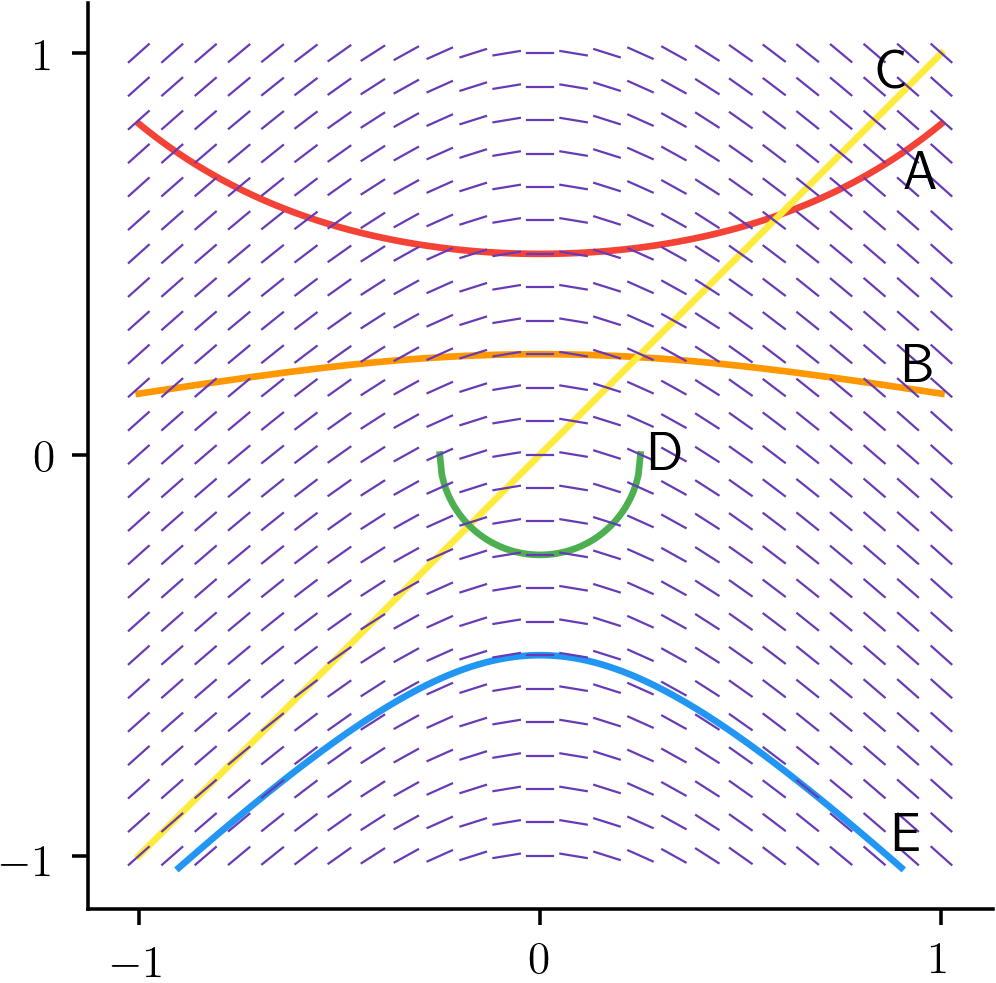
\includegraphics[width=4in]{images/slope01.png}
\end{image}\end{center}
\begin{multipleChoice}
\choice{A}
\choice{B}
\choice{C}
\choice{D}
\choice[correct]{E}
\end{multipleChoice}
\end{exercise}

\begin{exercise}
Which of the curves below is a solution of the ODE illustrated by the slope field?
\begin{center}\begin{image}
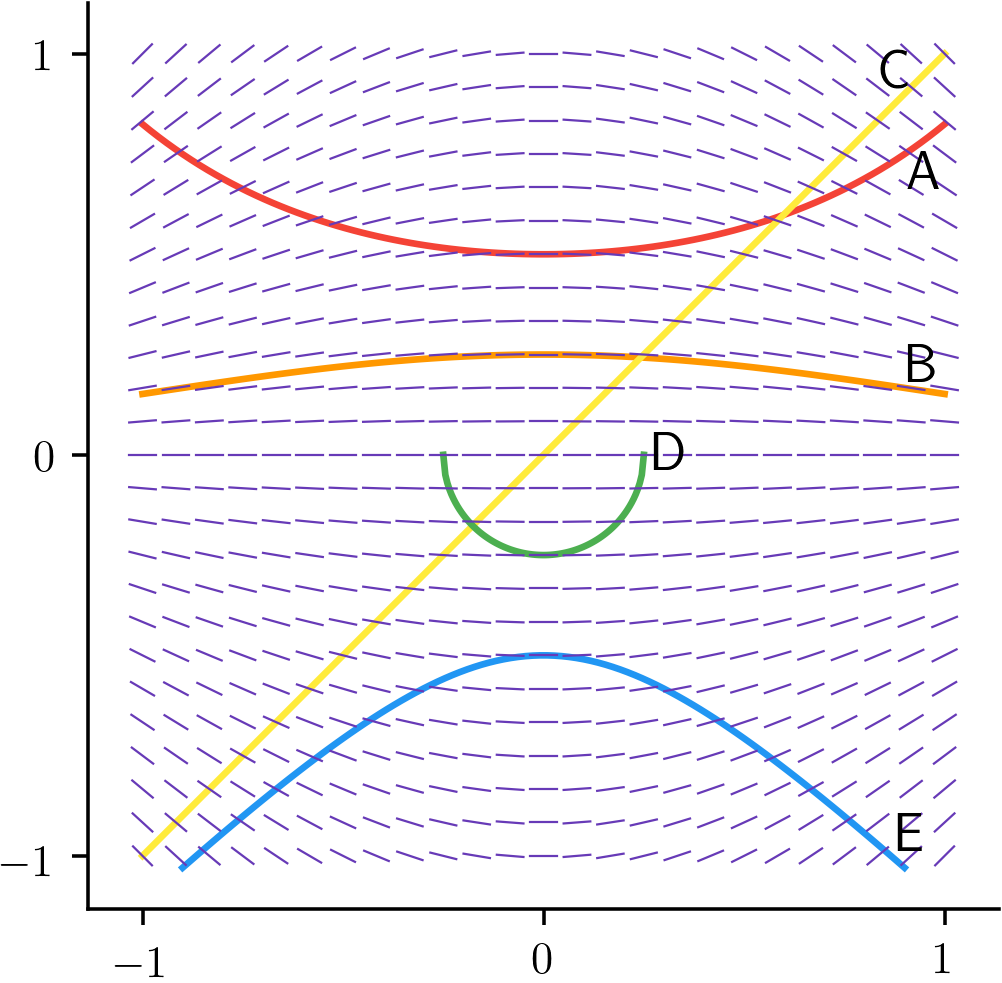
\includegraphics[width=4in]{images/slope02.png}
\end{image}\end{center}
\begin{multipleChoice}
\choice{A}
\choice[correct]{B}
\choice{C}
\choice{D}
\choice{E}
\end{multipleChoice}
\end{exercise}

\begin{exercise}
Trace the solution of the given ODE which begins at the point A. Which of the other labelled points will the solution pass through?
\begin{center}\begin{image}
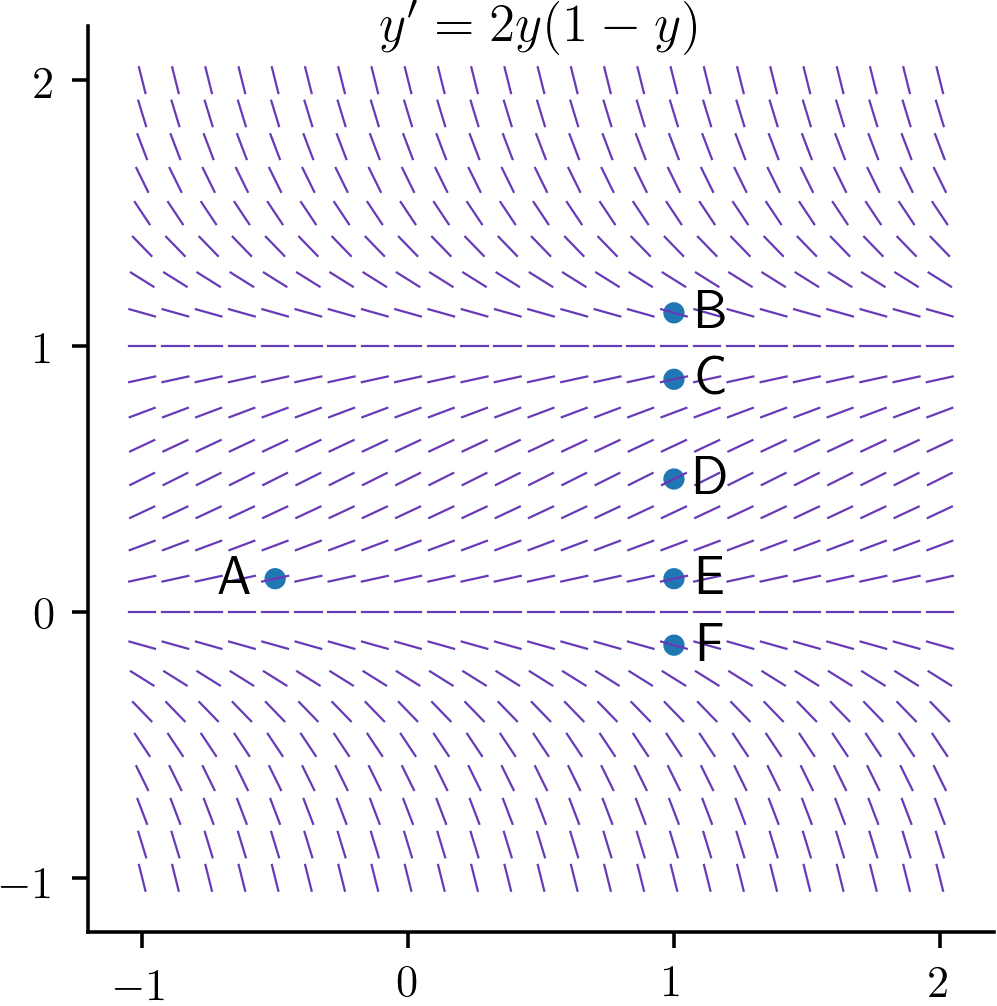
\includegraphics[width=4in]{images/connect01.png}
\end{image}\end{center}
\begin{multipleChoice}
\choice{B}
\choice[correct]{C}
\choice{D}
\choice{E}
\end{multipleChoice}
The ODE $y' = 2y (1-y)$ has one asymptotically stable constant solution. It is 
\[ y = \answer{1}. \]
\end{exercise}

\begin{exercise}
Trace the solution of the given ODE which begins at the point A. Which of the other labelled points will the solution pass through?
\begin{center}\begin{image}
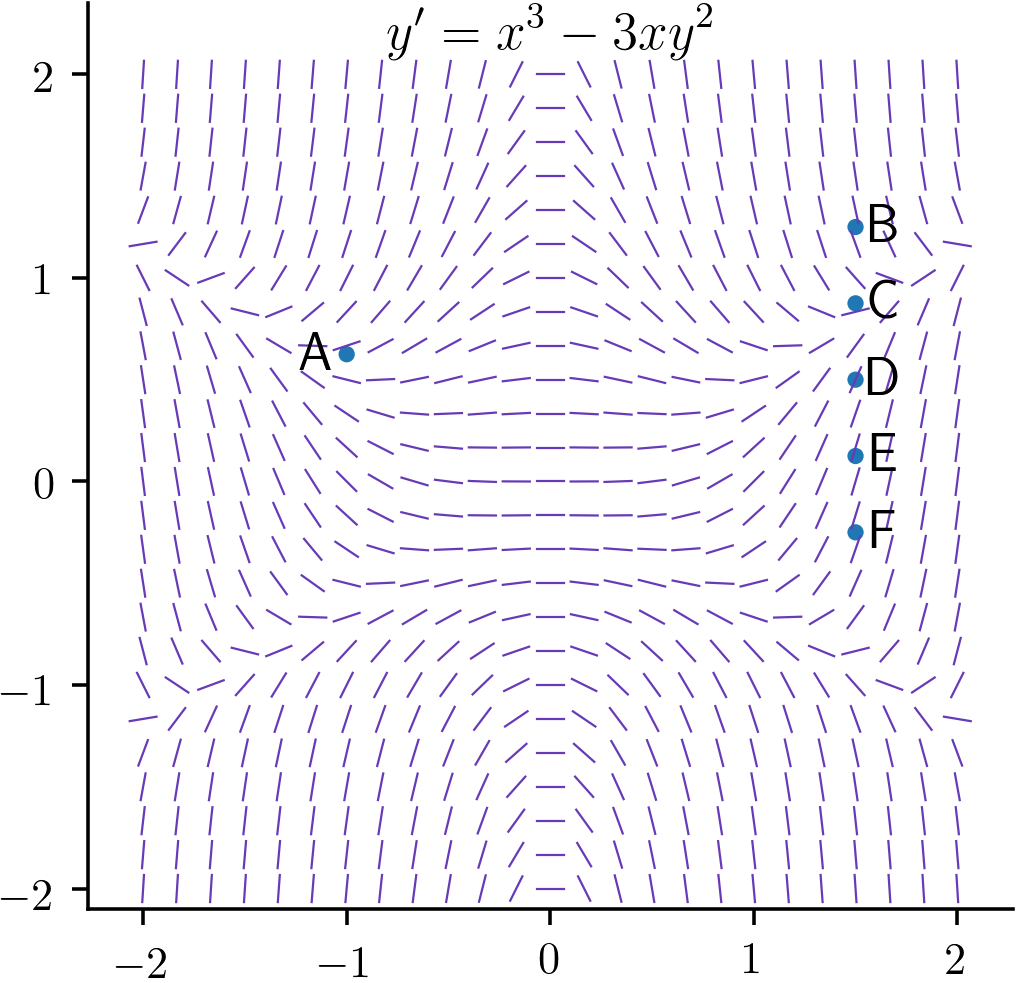
\includegraphics[width=4in]{images/connect02.png}
\end{image}\end{center}
\begin{multipleChoice}
\choice{B}
\choice[correct]{C}
\choice{D}
\choice{E}
\end{multipleChoice}
The ODE $y' = x^3 - 3x y^2$ has \wordChoice{\choice[correct]{no}\choice{one}\choice{two}\choice{three}} constant solutions.
\end{exercise}

\begin{exercise}
Let $y(x)$ be the solution to the initial value problem $y' = y$ with $y(0) = 1$. Use Euler's Method with step size $h = 1$ to approximate the value of $y(4)$. Fill in your work in the table below.
\begin{center}
\begin{tabular}{rrr}
$x$ & $y$  & $y + y h$ \\
\hline
$0$ & $1$  & $2$ \\
$1$ & $\answer{2}$  & $\answer{4}$ \\
$\answer{2}$ & $\answer{4}$  & $\answer{8}$ \\
$\answer{3}$ & $\answer{8}$ &  $\answer{16}$ \\
$\answer{4}$ & $\answer{16}$   &  \\
\end{tabular}
\end{center}
\[ y(4) \approx \answer{16}. \]
\end{exercise}

\begin{exercise}
Let $y(x)$ be the solution to the initial value problem $y' = x-y$ with $y(0) = 1$. Use Euler's Method with step size $h = 1$ to approximate the value of $y(5)$. Fill in your work in the table below.
\begin{center}
\begin{tabular}{cccc}
$x$ & $y$ & $(x - y)$ & $y + (x - y) h$ \\
\hline
$\answer{0}$ & $\answer{1}$ & $\answer{-1}$ & $\answer{0}$ \\
$\answer{1}$ & $\answer{0}$ & $\answer{1}$ & $\answer{1}$ \\
$\answer{2}$ & $\answer{1}$ & $\answer{1}$ & $\answer{2}$ \\
$\answer{3}$ & $\answer{2}$ & $\answer{1}$ & $\answer{3}$ \\
$\answer{4}$ & $\answer{3}$ & $\answer{1}$ & $\answer{4}$  \\
$\answer{5}$ & $\answer{4}$
\end{tabular}
\end{center}
\[ y(5) \approx \answer{4}. \]
Is the function $y = x-1$ a solution of the ODE $y' = x-y$?
\begin{multipleChoice}
\choice[correct]{Yes}
\choice{No}
\end{multipleChoice}
If yes, is it a solution of the IVP $y' = x-y$ and $y(0) = 1$?
\begin{multipleChoice}
\choice{Yes}
\choice[correct]{No}
\choice{Not applicable}
\end{multipleChoice}
Is the function $y = x -1 + 2 e^{-x}$ a solution of the IVP $y' = x-y$ and $y(0) = 1$?
\begin{multipleChoice}
\choice[correct]{Yes}
\choice{No}
\end{multipleChoice}
Given this, what is the difference between the approximated value of $y(5)$ that you calculated and the exact value. If you get a negative answer, take its absolute value:
\[ | y_{\text{approx}}(5) - y_{\text{exact}}(5)| = \answer{2 e^{-5}} \approx 0.0135. \]
\end{exercise}



\end{document}
